Um modelo de sistema prima intencionalmente pela abstração simplificada da descrição do sistema a ser desenvolvido, ressaltando as caracterísiticas mais importantes que o mesmo pode apresentar. O modelo conceitual é um modelo de sistema simples, usado para representar os conceitos em um domínio do problema. É um modelo de arquitetura de alto nível, geralmente expresso como diagramas de blocos simples, nos quais cada conceito é representado por um retângulo identificado, com linhas indicando as associações entre seus subsistemas \cite{Sommerville:Livro}.

O modelo conceitual também pode ser utilizado para representar a modelagem entidade-relacionamento de banco de dados relacionais. Nesse contexto, entidades do MER podem ser associadas como classes simplificadas de objetos (sem possuirem suas operações), atributos com atributos de classes e nas ralações como associações identificadas entre as classes \cite{Sommerville:Livro}. Na Figura \ref{fig:modeloConceitual}, podemos verificar como esse modelo de sistema é aplicado ao domínio do problema do LabInstru Web.

\begin{figure}[H]
	\centering
	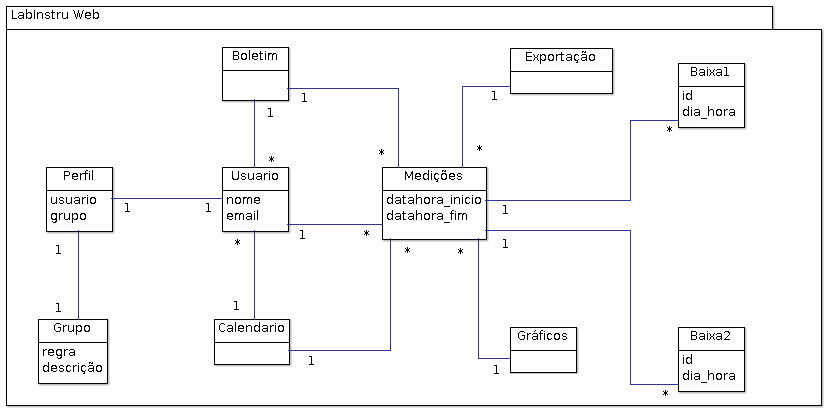
\includegraphics[scale=0.8]{img/ModeloConceitual.png}
	\caption{Módelo Conceitual - LabInstru Web.}
	\label{fig:modeloConceitual}
\end{figure}

No diagrama acima, podemos verificar que a entidade Usuário representa os atores responsáveis por interagir com a aplicação, o mesmo pode ser de um dos dois tipos: Admin ou User. O perfil de usuário Admin, possui privilégios especiais, como exemplo, ser apenas esse perfil capaz de alimentar a base de dados da aplicação com dados provenientes da estação meteorológica da est. Esse usuário administrador, também é o responsável em cadastrar e manter osusuários da plataforma web mencionada. O perfil de usuário User, poderá fazer sua autenticação por meio de um login, e utilizar as funcionalidades disponibilizadas pela aplicação, como as consultas às medições contidas no banco de dados da aplicação, exportação dessas consultas em um formato de dados específico (txt, csv, xml) ou exportação de gráficos referentes a essa determinada consulta. O Usuário User também pode solicitar a geração dos Boletins Meteorológicos, bem como os Calendários de Disponibilidades das medições persistidas na aplicação.

As entidades Baixa1 e Baixa2 representam as tabelas no banco de dados da aplicação, no qual, tais tabelas persistem os arquivos de texto no formato .dat gerados pela estação meteorológica da est. Essas duas entidades formam a base da aplicação web,  todas as consultas, exportações, gráficos, boletim meteorológico e calendário de disponibilidade são gerados a partir dessas bases de dados.